\documentclass[a4paper,12pt]{article}

% Packages
% Use Helvetica (Arial alternative)
% \usepackage{mathptmx} % Times-like font
% \renewcommand{\familydefault}{\sfdefault}
\usepackage{setspace}
\usepackage[utf8]{inputenc} % Encoding
\usepackage[T1]{fontenc}    % For output encoding
\usepackage[ngerman]{babel}
\usepackage{graphicx}       % For images
\usepackage{amsmath}        % For math equations
\usepackage{hyperref}       % For hyperlinks
\usepackage[a4paper, top=3cm, bottom=3cm, left=2.5cm, right=2cm]{geometry}
\usepackage{fancyhdr} %%Fancy Kopf- und Fußzeilen
\usepackage[backend=biber,style=authoryear]{biblatex}
\addbibresource{literatur.bib}

\onehalfspacing





% Document metadata
\title{Masterclass Assignment Title}
\author{Name: Franz Reitmayer \\ Immatrikulationsnummer: 444139}
\date{\today}

\begin{document}

% Title Page
\maketitle
\vfill
\begin{center}
\textbf{Studiengang: MBA Digital Management und Leadership} \\
AKAD University \\
Semester: Winter 24/25
\end{center}
\vfill
\newpage
\tableofcontents
\newpage


% Main Content
\section{Einleitung}
\subsection{Beschreibung des Themas}
\subsection{Abgrenzung Themas}
\subsection{Aufbau und Ablauf der Arbeit}


\section{Systemtheorie}
\subsection{Der Systembegriff}
\subsection{Klassifizierungen unterschiedlicher Systeme}\footnote{\cite{Ulrich2001}}
% \begin{figure}
% 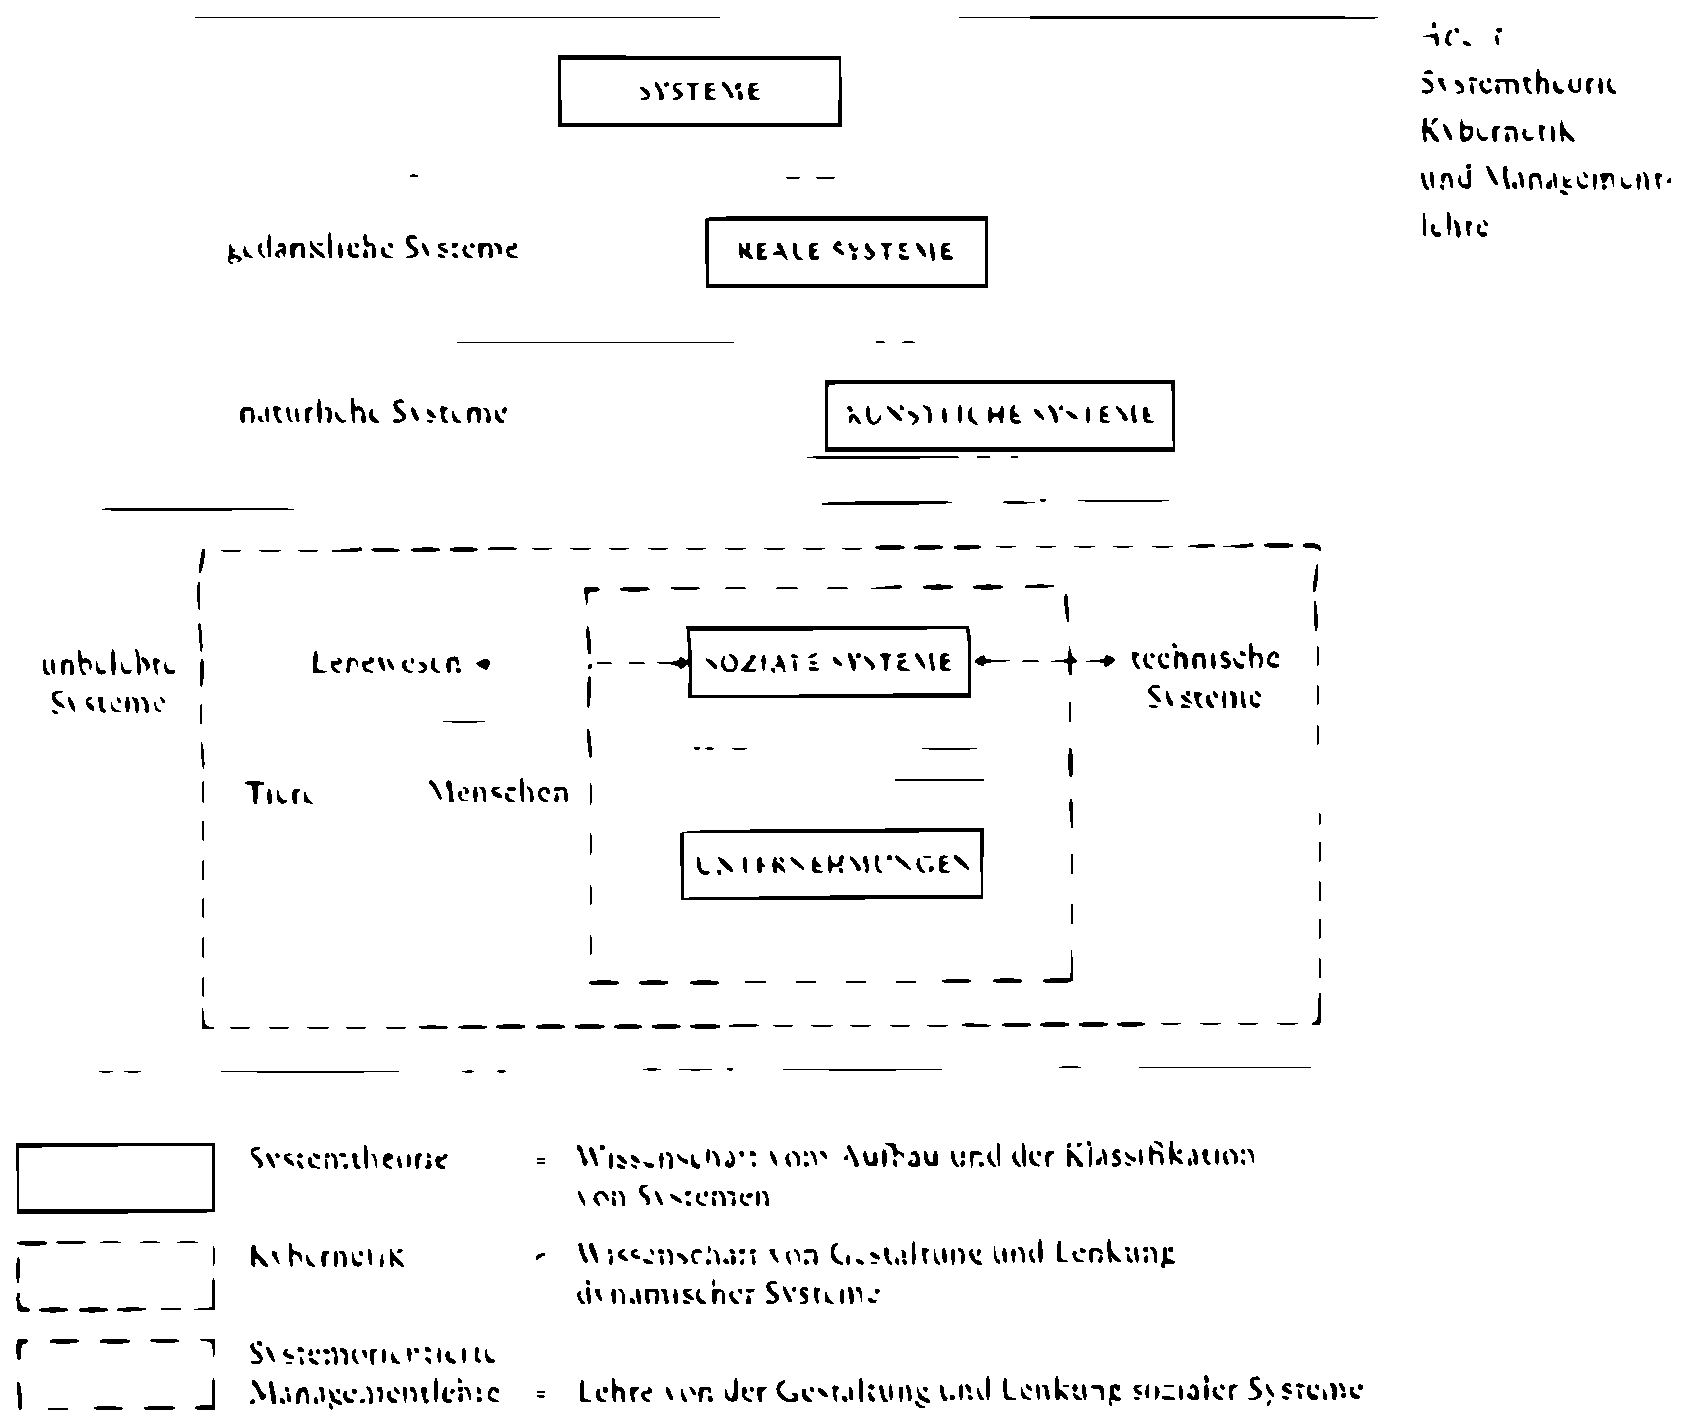
\includegraphics[width=0.8\textwidth]{systeme-ulrich.eps}
% \end{figure}                                                                                                                                                
\subsection{Unterschiedliche Systemtheorien}
\subsubsection{Allgemeine Systemtheorie nach Ludwig von Bertalanffy}
\subsubsection{Soziologische Systemtheorie nach Talcott Parsons}
\subsubsection{Soziologische Systemtheorie nach Niklas Luhmann}
\subsubsection{Systemtheorie des Unternehmens nach Hans Ulrich}
\subsubsection{Soziotechnische Systemtheorie nach Günther Ropohl}

\section{Argumentationspfade ??}
\subsection{Offene und geschlossene Systeme}
\subsection{Interdependenz}
\subsection{Selbstregulation}
\subsection{Autopoiesis}
\subsection{Differenzierung von System und Umwelt}
\subsection{Komplexitätsreduktion}
\subsection{Kommunikation als Hauptelement}
\subsection{Selbstreferenziell}
\subsection{Handlung}
\subsection{Funktionale Differenzierung}

\section{Kritische Einwände}
\subsection{Abstrakte Begriffswelt}
\subsection{Supertheorie vs. fehlende Einheitlichkeit}
\subsection{Fehlen Normativer Aussagen}
\subsection{Selbstdienlichkeit durch Selbstreferenzialität?}

\section{Fazit und Zusammenfassung}
\subsection{Fazit und Kritische Würdigung}
\subsection{Ausblick}


% References
\newpage

\nocite{*}
\printbibliography
% \bibliographystyle{plain}
%\bibliography{literatur}
% End of Document

\end{document}